\documentclass{article}
\usepackage{graphicx} % Required for inserting images
\usepackage{float}
\usepackage[a4paper, margin=1in]{geometry}
\usepackage{amsmath}
\usepackage{hyperref}
\usepackage{url}
\parindent 0pt

\title{GPS Coding and Wiring}
\author{Hritik Roy Chowdhury}
\date{October 2023}

\begin{document}

\maketitle

\section{Introduction}
This report will outline the wiring connections, circuitry, and programming for the NEO-6M GPS module to be used in the project. Note that this report is just one of the few methods and 
researches explored and carried out. This report will explain:
\begin{itemize}
    \item Wire the NEO-6M GPS module to the Arduino UNO
    \item Get raw GPS data
    \item Parse raw data to obtain selected and readable GPS information
    \item Get location
\end{itemize}
The majority of the information in this report is taken from a tutorial online explaining the NEO-6M GPS module's usage with the Arduino Uno 
\footnote{
Anon, (2018). \textit{Guide to NEO-6M GPS Module Arduino | Random Nerd Tutorials}. [online] Available at: \url{https://randomnerdtutorials.com/guide-to-neo-6m-gps-module-with-arduino/}.
}.

\section{Wiring}
Figure \ref{fig:connections} shows the simple wiring configurations to setup the GPS module for the Arduino. The GPS module uses a 5V supply to VCC and the transmitting and receiving pins go to their respective opposites on the Arduino. A ground is of course needed too.
\begin{figure}[H]
    \centering
    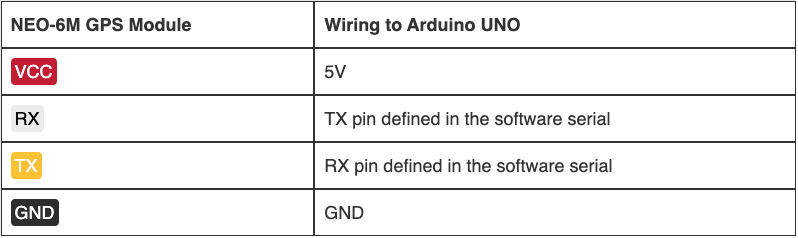
\includegraphics[width=\textwidth]{connections.png}
    \caption{Wiring for the GPS to the Arduino}
    \label{fig:connections}
\end{figure}



\end{document}
